\chapter{Implemenations and Evaluations}

\section{Experiments}
An extensive set of experiments are carefully performed and monitored to assess the effectiveness of the models and methodologies using serveral metrics, data sources, and model architectures.

\subsection{Datasets}
\subsubsection{Flickr8k}
Flickr8K was first proposed by \cite{Hodosh:2013:FID:2566972.2566993} as a benchmark collection for sentence-based image description and search. The dataset consists of $8,000$ images accompanied with five different description sentences which provide clear description of salient entities and events. \textit{TODO: re-paraphrase}
\subsubsection{Flickr30k}
As introduced in \cite{DBLP:journals/tacl/YoungLHH14}, Flickr30k is an extension of Flickr8k. The dataset is comprised of $158,915$ crowd-sourced captions describing $31,783$ images. Except for images that overlapped in Flickr8k, the new images and captions in this dataset focus on people involved in everyday activities and events.

Several examples of images and captions in Flickr8K and Flickr30k are shown in figure \ref{fig:flickr-examples}.

\begin{figure}
	\centering
	\label{fig:flickr-examples}
	\begin{tabular}{l l}
		\toprule
		\multirow{5}{*}{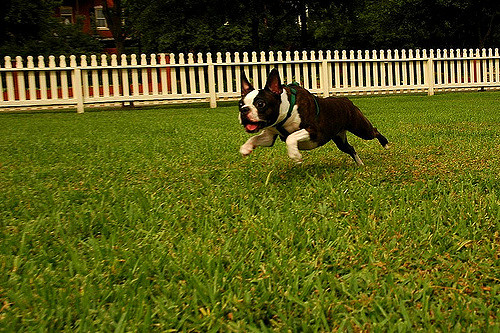
\includegraphics[width=0.25\linewidth]{Chapters/Fig/black_dog_running_fence.jpg}} & \parbox{11cm}{\small{A black and white dog is running in a grassy garden surrounded by a white fence}} \\
		& \small{A black and white dog is running through the grass} \\
		& \small{A Boston terrier is running in the grass} \\
		& \small{A Boston Terrier is running on lush green grass in front of a white fence} \\
		& \small{A dog runs on the green grass near a wooden fence} \\
		\midrule
		\begin{minipage}{0.25\linewidth}
			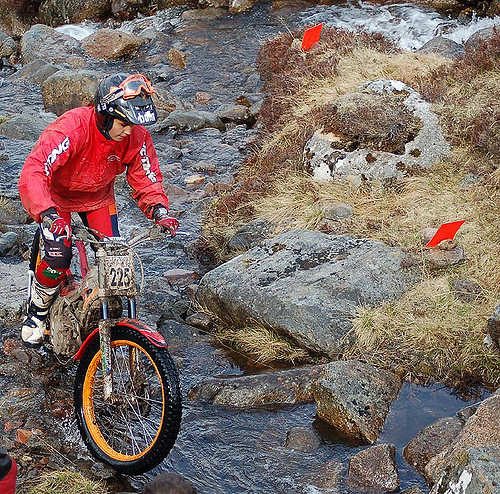
\includegraphics[width=\linewidth]{Chapters/Fig/men_red_helmet_riding_bike_rocks.jpg}
		\end{minipage}
		&
		\begin{minipage}{0.75\linewidth}
			\parbox{11cm}{\small{A boy in a black helmet and red long sleeve shirt rides his motorbike over a rocky stream}} \\
			\small{A man on a motorcycle steers through swampy terrain} \\
			\small{A man rides his bike over rocks and a creek.} \\
			\small{A motocross bike is being ridden between markers in a running stream.} \\
			\small{A person is dirt biking over rocks and water.}
		\end{minipage}\\
		\midrule
		\begin{minipage}{0.25\linewidth}
		IMAGE 335110163
			% \includegraphics[width=\linewidth]{Chapters/Fig/woman_photograph.png}
		\end{minipage}
		&
		\begin{minipage}{0.75\linewidth}
			\parbox{11cm}{\small{A woman with dark hair and a white shirt is taking a picture of an object at close range }} \\
			\parbox{11cm}{\small{A photographer taking a closeup photo of a glass perfume jar }} \\
			\parbox{11cm}{\small{A woman taking picture of her pet in her home }} \\
			\parbox{11cm}{\small{A woman taking a photo of an object on a bed }} \\
			\parbox{11cm}{\small{The lady is taking a closeup picture }} \\
		\end{minipage}\\
		\begin{minipage}{0.25\linewidth}
		IMAGE 908636680
			% \includegraphics[width=\linewidth]{Chapters/Fig/woman_photograph.png}
		\end{minipage}
		&
		\begin{minipage}{0.75\linewidth}
			\parbox{11cm}{\small{A group of eight campers sit around a fire pit trying to roast marshmallows on their sticks}} \\s
			\parbox{11cm}{\small{A group of men and women surrounding a bonfire while having conversation }} \\
			\parbox{11cm}{\small{Several people having fun and toasting marshmallows around a campfire }} \\
			\parbox{11cm}{\small{A group of people are outside , roasting marshmallows in a fire }} \\
			\parbox{11cm}{\small{Seven adults sit around a fire pit having a conversation }} \\
		\end{minipage}\\
		\bottomrule
	\end{tabular}
	\caption{Images with 5 crowd-sourced captions in Flickr8k and Flickr30k}
\end{figure}
\subsubsection{MSCOCO}
MSCOCO \cite{DBLP:journals/corr/LinMBHPRDZ14} (Microsoft Common Objects in Context) is a large-scale dataset that addresses three core research problems in scene understanding: detecting non-iconic views of objects, contextual reasoning between objects and the precise 2D localization of objects. It has been considered as the start-of-the-art dataset for numerous computer vision tasks (e.g., image classification, object detection, object segmentation, scene labelling, etc.). The dataset has approximately $328,000$ images of complex everyday scenes containing common objects in their natural context. Like in aforementioned Flickr8k \& Flickr30k datasets, each images in MSCOCO is also associated with five caption sentences that describe the content of such image.

The statistics of the datasets are summarized in table \ref{tab:dataset-statistics}
\begin{table}
	\centering
	\label{tab:dataset-statistics}
	\begin{tabular}{l|c|c|c}
		\toprule
		\multirow{2}{*}{Dataset name} & \multicolumn{3}{c}{size} \\ \cline{2-4}
		& train & validation & test \\ \midrule
		Flickr8k & 6000 & 1000 & 1000 \\
		Flickr30K & 28000 & 1000 & 1000 \\
		MSCOCO & 82783 & 40504 & 40775 \\
		\bottomrule
	\end{tabular}
	\caption{Dataset statistics}
\end{table}
\subsection{Environment}
	\subsection{Hardware configurations}
	\subsection{Software}

\subsection{Experiment 1}{: Compare the effect of different receptive field sizes to the accuracy of vision model in classification task}

\section{Evaluations}

\subsection{Evaluation metrics}
	\subsubsection{Human raters}
	Although it is sometimes not clear whether a description should be deemed successful or not given an image, many researches have proposed several evaluation metrics. The most reliable (but time consuming) is to ask for raters to give a subjective score on the usefulness of each description given the image. In this thesis, this method was used to reinforce that some of the automatic metrics indeed correlate with this subjective score, following the guidelines proposed in \cite{Hodosh:2013:FID:2566972.2566993}, which asks the graders to evaluate each generated senetence with a scale from 1 to 4. Specifically, the rates are asked whether the image is described without any errors, described with minor errors, with a somewhat related description, or with an unrelated description, with a score of 4 being the best and 1 being the worst.

	For this metric, we set up an Amazon Mechanical Turk experiment. Each image was rated by 2 workers. The typical level of agreement between workers is 65\%. In case of disagreement, we simply average the scores and record the average as the score. For variance analysis, we perform bootstrapping (re-sampling the results with replacement and computing means/standard deviation over the resampled results.). Like \cite{Hodosh:2013:FID:2566972.2566993} we report the fraction of scores which are larger or equal than a set of predefined thresholds.